\chapter{Microgrid Protection} 
\label{ch:microgrid_protection}
\section{Introduction}
% Increased integration of DERs, such as generation units and energy storage systems, at the distribution level,  behind the meter, gives opportunities to operate areas of power networks independently from the main grid to maintain power supply during disruptions to the main grid, such as faults or equipment failures, as Microgrids.These systems, however, present unique protection challenges to detect and respond to faults. This chapter explores the key protection issues associated with microgrids and discusses possible strategies to address them. 

Modern microgrids integrate multiple distributed energy resources (DERs) such as photovoltaic (PV), wind, battery energy storage systems (BESS), and diesel generators. 
Unlike conventional radial feeders, microgrids are \emph{active networks} where fault currents are limited, directional, and dependent on the converter control strategy. 
This chapter extends the protection concepts developed for distributed power systems to coordinated multi–source microgrids, addressing their architectures, operating modes, design considerations, challenges, and the proposed four–level protection framework.


\section{Microgrid architectures and types} 

A microgrid comprises a collection of distributed energy resources (DERs) and electrical loads interconnected within a well-defined boundary. It is a unified and controllable system that can coordinate with the primary grid or operate independently in islanded mode. This concept aligns with the definition provided by the U.S. Department of Energy (DOE).
Microgrids are typically connected to the main power grid at distribution or sub-transmission levels, with their capacity limited by equipment ratings. Common applications include campuses, industrial parks, communities, military bases, and hospitals, with sizes ranging from a few kilowatts to tens of megawatts.

\subsection{Types of Microgrid}
Microgrids can be classified according to network configuration and coupling medium:
\begin{itemize}
    \item \textbf{AC microgrids:} most common due to compatibility with traditional power systems.
    \item \textbf{DC microgrids:} offering enhanced control and reliability.
    \item \textbf{Hybrid AC–DC microgrids:} combining both AC and DC features.
\end{itemize}

This work focuses specifically on protection strategies for AC microgrids.

\begin{figure}[!ht]
	\centering
	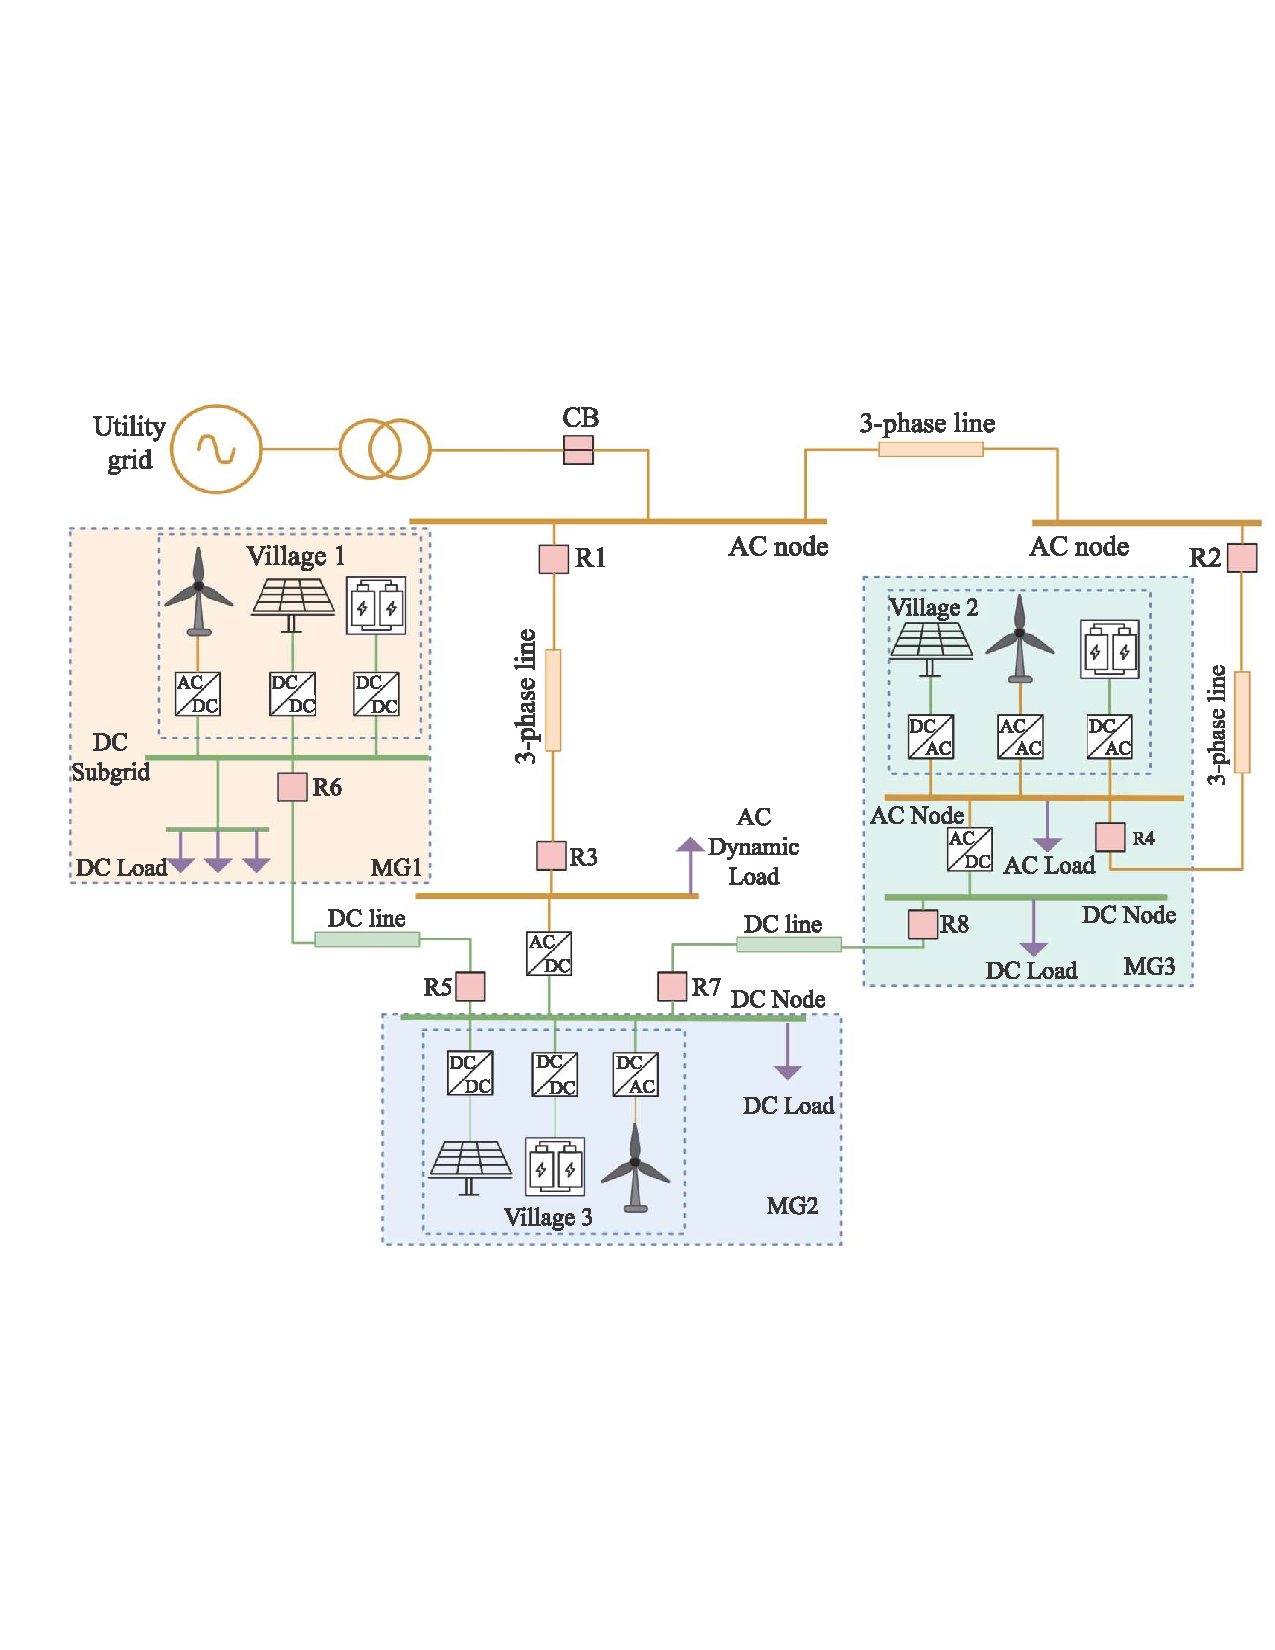
\includegraphics[width=0.75\columnwidth]{images/chapter_4/Microgrid.pdf}
	\caption{Practical Microgrid.}
	\label{fig_MG}
\end{figure}

\subsection{Modes of Operation}

A microgrid can operate in three distinct modes:
\begin{enumerate}
    \item \textbf{Grid–connected:} fault current dominated by the main grid; DERs contribute through current–limited converters.
    \item \textbf{Islanded:} current magnitude and waveform determined by inverter controls and internal impedance.
    \item \textbf{Transition:} dynamic period between grid–connected and islanded; topology and control references change.
\end{enumerate}

\subsubsection{Variation in fault current under each mode}

The instantaneous fault current of an inverter–based resource can be expressed as:
\begin{equation}
i_f(t) = I_{max} \sin(\omega t + \theta_f)
\label{eq:if_time}
\end{equation}
where $I_{max}$ is the current–limit imposed by the converter controller (typically $1.2$–$2.0$\,pu) and $\theta_f$ is the fault current phase angle relative to the grid voltage.
The peak fault current therefore varies by control mode:
\begin{equation}
I_{f,grid} > I_{f,trans} > I_{f,island} \quad [\text{A}]
\label{eq:if_levels}
\end{equation}
indicating reduced magnitude and altered phase response during islanded operation.


% Microgrids may operate grid-isolated or grid-interconnected. There is also a transition from grid-isolated operation to grid-interconnected operation and from grid-interconnected operation to grid-isolated operation.







\section{Design Considerations}


\begin{enumerate}
	\item Define zones of protection - protection devices

	 \item Selection of Protection Schemes.
      \item Communication infrastructure.
    \item  Additional functions. 
    \item System Grounding Considerations

\end{enumerate}

\subsection{System Studies for Microgrid Design}

\begin{enumerate}
	\item Pickup threshold (Detection requirement)
	 \item Tripping time (Coordination requirement)
\end{enumerate}


Protection coordination in microgrids requires \textit{multi–scenario system studies}.  
Each mode must be analysed for short–circuit level, directionality, and relay reach.

The Thevenin equivalent at the point of common coupling (PCC) determines the prospective fault current:
\begin{equation}
I_{sc} = \frac{E_{th}}{Z_{th}} = \frac{V_{pcc}}{R_{eq} + j X_{eq}}
\label{eq:isc}
\end{equation}
where $Z_{th}$ varies dynamically as DERs connect or disconnect. 

\subsection{Protection in grid-connected, islanded, and transition modes}
Protection challenges in microgrids can generally be grouped into three key areas:
\begin{enumerate}
    \item Disconnecting the microgrid from the primary electrical power system (EPS) in response to de-energisation, faults, or other abnormal grid conditions.
    \item Reconnecting and synchronising the microgrid with the EPS, and detecting and isolating faults or abnormal conditions within the microgrid, operating in islanded mode or connected to the primary grid.
\end{enumerate}


\subsubsection{Microgrid Protection During Grid-Isolated Operation}
Protection strategies must address short circuits, abnormal conditions, and power balance in grid-isolated microgrids. Operating independently from the primary grid often results in lower available fault currents, necessitating adjustments in protection coordination. Protection schemes are adapted to ensure system reliability in this mode.
Short-circuit protection is crucial for isolating faulty components such as rotating machines, inverters, transformers, buses, cables, and lines. In grid-isolated conditions, conventional protection may need enhancements for improved sensitivity and selectivity. 

% Directional elements, logical combinations, and communication-assisted protection enhance fault detection and coordination.
% For rotating machinery, guidance is available in IEEE standards such as Std 242, C37.96, C37.102, and C37.101. Inverter-based systems follow IEEE Std 1547 and UL 1741 for interconnection and self-protection.
% Frequency (81) and voltage protection (27, 59) are employed to maintain load-generation balance. Overfrequency (81O) or underfrequency (81U) can disconnect generation or load, respectively. Similarly, overvoltage (59) or undervoltage (27) protection may act on capacitor banks or inductive loads.
% Re-synchronization protection when reconnecting to the grid involves voltage and frequency monitoring at points of common coupling using devices 59, 27, 81O, and 81U. Synchronizing (25) and Auto-Synchronizing (25A) elements ensure safe reconnection by verifying phase alignment and system stability. Where multiple reconnection points exist, careful sequencing can optimize the number and type of synchronizing elements required.

\subsubsection{Microgrid Protection During Grid-Interconnected Operation}
In grid-interconnected mode, microgrid protection focuses on two main areas: internal microgrid protection and re-synchronization with the main power system (EPS). While internal protection methods remain similar to those used in islanded mode, coordination with EPS protection becomes essential, making coordination the primary challenge rather than fault detection.
Re-synchronization protection includes directional elements at points of common coupling to ensure safe reconnection. 

\subsection{Grounding Considerations}
Grounding configuration affects zero–sequence impedance $Z_0$ and therefore the residual current:
\begin{equation}
I_0 = \frac{3V_0}{Z_0} = \frac{V_{an}+V_{bn}+V_{cn}}{Z_0}
\label{eq:groundcurrent}
\end{equation}
In isolated or high–resistance grounded systems, $I_0$ becomes too small for conventional earth–fault relays; voltage–based detection or sensitive differential protection is required.

\subsection{Communication System}
\textbf{IEC\,61850\,GOOSE} messaging enables exchange of \emph{Trip/Block} and \emph{Transfer–Trip} signals with latencies below $4$\,ms.  
This is vital to maintain selectivity in low–current islanded faults.

\subsection{Resynchronization}
When a microgrid with AC PCC connection(s) is operating grid-isolated, a synchronization process may be needed prior to microgrid re-synchronization to the EPS. Synchronization considerations with AC connection at the PCC include:

\subsection{Impact of Microgrid Control Strategy on Protection}

The fault current behaviour is governed by the inverter control algorithm.
For a grid–following (GFL) inverter:
\begin{equation}
\mathbf{I}_{dq}^* = K_p(\mathbf{V}_{dq}^{ref} - \mathbf{V}_{dq}) + K_i \int (\mathbf{V}_{dq}^{ref} - \mathbf{V}_{dq})\,dt
\label{eq:gflcurrent}
\end{equation}
During faults, the current controller saturates at $I_{max}$ and limits fault contribution.  
Grid–forming (GFM) inverters instead impose a voltage reference:
\begin{equation}
\mathbf{V}_{dq}^* = \mathbf{V}_{dq}^{nom} - R_v \mathbf{I}_d - L_v \frac{d\mathbf{I}_d}{dt}
\label{eq:gfmvoltage}
\end{equation}
Thus, $I_f$ depends on virtual impedance parameters $(R_v,L_v)$, resulting in smaller fault currents than synchronous machines.




A microgrid must function as a single controllable unit from the grid's perspective. Its control system—whether centralized or distributed—comprises hardware, software, or both, and is responsible for monitoring grid conditions and managing microgrid operations to meet specific performance goals. These goals typically include minimizing outages for critical loads, reducing greenhouse gas emissions, and improving energy efficiency.
To achieve these objectives, the control system handles tasks such as voltage and frequency regulation, load management, islanding and re-synchronization, power flow control, and operational optimization. Intelligent control and distribution automation (DA) schemes enhance microgrid performance and protection. Key examples include:

\begin{enumerate}
\item FLISR (Fault Location, Isolation, and Service Restoration)
\item Automated load transfer and reconfiguration
\item Rapid/emergency load shedding
\item Integrated Volt/VAR control (IVVC) and optimization
\end{enumerate}

These control strategies directly influence the design and coordination of protection systems within a microgrid. Advanced microgrid control systems play a critical role in optimizing performance and reliability, but they also introduce challenges for protection. These control systems, often organized in a hierarchical structure (primary, secondary, tertiary), manage various tasks including energy management, fault isolation, load balancing, voltage/frequency regulation, and system reconfiguration.
\subsubsection{Key Challenges and Considerations:}
Dynamic Operating Conditions: Microgrid conditions change frequently due to DER variability, load fluctuations, and reconfiguration. This results in variable fault current levels, complicating protection coordination.\\

Circuit Reconfiguration:Automatic or manual reconfiguration enhances system reliability (e.g., by rerouting power) but affects fault current levels and directions. Protection settings must be adaptable to these changes.\\

\subsection{Protective Equipment}



Common protection methods include:

\begin{enumerate}
	\item Phase Overcurrent (50/51) for phase faults
	\item Ground Overcurrent (50N/50G/51N/51G) and Negative-Sequence Overcurrent (46) for ground and phase imbalances
	\item Ground Overvoltage (59N) for high-impedance or ungrounded systems
         \item Voltage-Restrained/Controlled Overcurrent (51VR/51VC) for low-current fault detection.
          \item  Differential Protection (87) for transformers (87T), buses (87B), and lines (87L)
    
\end{enumerate}

Key protection functions in this mode include:

\begin{enumerate}

\item Real and reactive power monitoring (IEEE devices 32, 32U, 32Q, 32QU) for power agreement enforcement and loss-of-grid detection.

\item Directional overcurrent protection (IEEE devices 67P, 67Q, 67N) for identifying faults on the EPS by detecting abnormal current flow from the microgrid toward the main grid.

\end{enumerate}


IEDs must support:
\begin{itemize}
    \item Multi–setting groups (grid/interconnected, islanded)
    \item Negative– and zero–sequence directional elements
    \item Voltage–restrained overcurrent (51V)
    \item Frequency and ROCOF elements for islanding detection
\end{itemize}



\section{Challenges in Microgrid Protection}
\begin{itemize}
    \item \textbf{Variable fault current levels} due to converter limits and grid strength.
    \item \textbf{Bidirectional fault current flow} from multiple DERs.
    \item \textbf{Loss of selectivity} as traditional time–grading fails under mode change.
    \item \textbf{Dependability across modes:} relays must operate both in grid–connected and islanded operation.
    \item \textbf{Maintaining DER availability} without over–tripping.
    \item \textbf{Detection of loss of grid (islanding)} within IEEE~1547 time constraints.
    \item \textbf{Resynchronisation} after fault clearance—requires sync–check and ROCOF supervision.
\end{itemize}


Changes in loading and fault levels can affect overcurrent protection.\\
Generator dispatch alters available fault current.\\
Reverse power flow can cause misoperation in non-directional protection.\\
Close-transition switching may temporarily increase fault currents.\\
Protection zones may need to be redefined based on the new topology.\\
Re-synchronization Considerations: When transitioning from islanded to grid-connected mode, synchronization is essential—especially in systems with rotating machines. Inverter-based systems may tolerate out-of-phase re-energization, but rotating machinery cannot and requires proper synchronization protection like sync check relays to avoid equipment damage.

Due to the unique characteristics of microgrids—such as variable fault current levels, bidirectional power flow, and operation in both grid-connected and islanded modes—traditional protection schemes often fall short. Customized and adaptive protection strategies, often involving communication and real-time data, are essential to ensure reliability and safety.




\section{Microgrid Protection System Design Considerations}








\section{Challenges of Microgrid Protection}

Microgrids pose distinct challenges for protection system design due to their dynamic configurations, shorter electrical distances, and high penetration of inverter-based generation. These inverters often produce low fault currents and may lack zero- or negative-sequence components, making traditional fault detection and directional protection difficult—especially in islanded mode.
The diversity in microgrid architectures further complicates protection, often requiring custom solutions. While general control and protection standards exist, dedicated standards specific to microgrid protection are still needed.
Key challenges in microgrid protection include:

\begin{enumerate}
	\item Variable fault current levels.
	\item Fault current contributions from inverter-based sources.
\item Sympathetic tripping
 \item Maintaining dependability for both modes of operation.
\item Maintaining source available after events Isolating fault currents
	 from all generating sources.
\item Impacts of micro grid control strategy on protection.
\item Topology changes.
\item Synchronization. 

\end{enumerate}

Additionally, microgrids often operate with low inertia and sensitive loads, demanding fast, reliable fault detection. When communication-based protection is used, low-latency communication becomes essential.


\subsubsection{Variable Fault Current Levels}

Variable Fault Current Levels are a major protection challenge in microgrids due to the diverse nature of fault current contributions from various sources such as synchronous generators, induction machines, and inverter-based DERs (e.g., renewables, EVs, storage systems).
Synchronous generators and induction machines provide fault currents that decay over time, with significantly lower magnitudes in islanded mode than when connected to the grid. This variation complicates coordination of protective devices across operating modes.\\

1. Inverter-based DERs Fault Current Contribution\\
Inverter-based DERs, however, behave very differently. Their fault current is typically limited to near-rated values and controlled within two cycles, often accompanied by high-frequency transients. Unlike traditional sources, inverters may not provide zero- or negative-sequence currents, and their ungrounded nature can further limit fault detection capability, particularly during unbalanced or non-ground faults. Smart inverters can alter power factor during faults, leading to fault currents with phase angles that differ from those of grid-supplied faults. These characteristics hinder the effectiveness of traditional overcurrent-based protection schemes.

\subsubsection{Maintaining Dependability for Grid-Interconnected and Grid-Isolated Mode} 

Operating DERs in parallel with the utility system requires consideration of how protection should respond to an event on the utility system. If a fault occurs on the utility system, local DERs may contribute to this fault. The DER contributions must be isolated from the fault. However, it may be desirable that the resource is available to restore power to a grid-isolated system if the fault causes an outage. This necessitates a coordination between DER protection and point of common coupling (PCC) protection if seamless formation of an island is of interest. Further, the DER may have the capability to ride through specified disturbances.


\subsubsection{Bidirectional Fault Current Flow}
 In microgrids, fault currents can flow in both directions depending on the fault location, making protection coordination more complex. This bidirectional flow impacts protection selectivity, DER availability, and fault isolation. Determining fault direction is especially difficult with inverter-based DERs due to their frequency response characteristics and low fault current levels.

\subsubsection{Protection Selectivity Considering Bidirectional Fault Current Flow}
 Protection systems must account for the direction of fault current to ensure selective tripping. Directional sensing equipment and protection strategies are essential, particularly with inverter-based sources that challenge traditional detection methods.\\

\subsubsection{Maintaining DER Availability After Events}
 DERs may contribute to utility-side faults, so coordination between DER protection and point-of-common-coupling (PCC) protection is necessary. It is often desirable to retain DERs for islanded operation post-fault, requiring relays to avoid unnecessary tripping during temporary disturbances.
Isolating Faults from All Generation Sources To fully clear a fault, contributions from all generation sources must be isolated. Even inactive DERs must be prevented from re-energizing faulted components, often necessitating lockout functions on their associated breakers.\\

\subsubsection{Isolating Fault Contributions From All Generation Sources}
A fault must be isolated from all generation sources for the fault to be cleared. When generation resources are interconnected and operating, their contributions to the fault may be detected and isolated. However, when resources are not connected, it may be desirable for the protection system 
to ensure that they cannot attempt to energize a faulted component. For example, consider the example system shown in Figure 9 with DER 1 and DER 2 not operating.

\subsubsection{Detecting Loss of Grid}
 Protective relays play a key role in identifying grid outages and initiating islanded operation. Common methods include reverse power and directional overcurrent detection. However, these may fail under low DER fault contributions or single-phase open conditions. \\
 
 1. Methods to detect grid faults.\\
 Solutions include direct transfer trip and zero- or negative-sequence voltage measurements.\\
2. Detecting Grid Outages.\\
 Undervoltage, overvoltage, frequency deviations, and their rates of change are used to detect grid loss. However, when DER generation matches load, a "non-detection zone" may exist. Advanced techniques such as synchrophasor-based detection or direct transfer trip are needed to ensure safe disconnection.\\
Handling Temporary Grid Faults.\\
 Deciding whether to ride through or isolate during temporary faults depends on DER capacity and operational mode. Quick isolation is needed if on-site resources can support the load, but in systems with delayed DER startup, riding through may prevent unnecessary outages. Coordination with automatic reclosing schemes is critical to avoid out-of-sync reconnections. For grids prone to temporary faults, operators may choose to proactively island based on forecasted conditions.

\section{Protection Scheme Solutions}.

Table~\ref{tab:schemes} summarises the applicable schemes.

\begin{table}[h!]
\centering
\caption{Comparison of microgrid protection schemes}
\label{tab:schemes}
\begin{tabular}{|l|c|c|c|}
\hline
\textbf{Scheme} & \textbf{Dependability} & \textbf{Selectivity} & \textbf{Comments} \\ \hline
Negative/Zero–Seq OC (51N/51G) & High (solid–grounded) & Moderate & Sensitive earth faults \\
Voltage–restrained OC (51V) & High & High & Effective under low currents \\
Under–Voltage (27) & Moderate & Low & Poor discrimination \\
Directional Interlocking & High & High & Bidirectional coordination \\
Comms–based Differential & Very High & Very High & Needs reliable channel \\
Bus Differential (87B) & Very High & Very High & Zone–specific \\
Centralised Detection & High & High & Requires redundant controller \\
\hline
\end{tabular}
\end{table}

\subsection{Adaptive Relay Settings}
Relay pickup is adjusted using voltage–dependent logic:
\begin{equation}
I_{pickup} = k_V \frac{V_{meas}}{V_{nom}} I_{nom}
\label{eq:adaptive}
\end{equation}
where $k_V$ (0.6–1.0) scales sensitivity with local voltage depression, ensuring reliable tripping in both grid–connected and islanded modes.

\subsection{Directional Interlocking}
For a pair of relays $R_1$ and $R_2$ on adjacent feeders, the coordination condition is:
\begin{equation}
t_{R_2} - t_{R_1} \ge \Delta T_c
\label{eq:coordination}
\end{equation}
where $\Delta T_c$ is the coordination interval (typically $0.3$–$0.5$\,s).  
In low–inertia microgrids, communication–assisted blocking using IEC\,61850 reduces $\Delta T_c$ to below $50$\,ms.

\subsection{Voltage–Restrained Overcurrent (51V)}
The operating current threshold varies inversely with voltage:
\begin{equation}
I_{op} = I_{set}\left(\frac{V_{nom}}{V_{meas}}\right)^n
\label{eq:51v}
\end{equation}
where $n$ (0.5–1.0) defines sensitivity to voltage sag.  
This maintains operation under low fault currents when $V_{meas}$ drops.



\subsection{Negative and Zero Sequence Overcurrent}
Used for detecting unbalanced faults where conventional phase overcurrent protection may be inadequate.\\
Effectiveness depends on DERs’ ability to generate negative/zero-sequence currents.\\
Limited in inverter-based systems.\\
\subsection{Under-Voltage Protection}
Detects faults by monitoring voltage drops.\\
Independent of fault current magnitude/direction.\\
Susceptible to misoperation during load switching and lacks selectivity.

\subsection{Voltage-Restrained/Controlled Overcurrent}
Enhances fault detection sensitivity in low fault current conditions.\\
Suitable for microgrids with inverter-based DERs.\\
Coordination and selectivity remain challenging.

\subsection{Adaptive Relay Settings}
Two Approaches: Pre-calculated Trusted Settings: Offline settings for known configurations; relies on condition monitoring to switch settings.\\
Near-Real-Time Calculations: Continuously adjusts settings based on real-time data; offers flexibility but adds complexity in modeling and testing.\\
Challenges: Protection gaps during transitions, synchronization issues, and communication failures.
\subsection{Transfer Trip and Operating Status Signals}
Use communication to send trip commands across devices, preventing unintentional islanding and coordinating DER protection.\\
Feeder relays can adjust behavior based on microgrid status.

\subsection{Directional Interlocking}
Proven, cost-effective scheme using directional logic or GOOSE messaging to detect and isolate faults in radial systems.

\subsection{Communication-Based Differential and Directional Blocking}
High-speed communication enables precise, mode-independent protection.\\
Effective for short line distances common in microgrids.\\
Differential protection is more sensitive, but both face challenges with tapped loads.
\subsection{Bus Differential Protection}
High or low impedance schemes protect specific bus zones.\\
Low-impedance preferred for varied CT ratios; more flexible with modern relays.
\subsection{Centralized Fault Detection System}
Aggregates data from IEDs and relays across the microgrid.
Enables faster fault location, isolation, and service restoration.
Two implementation methods:
Local fault clearing followed by centralized restoration coordination.
Real-time central fault detection and trip signal dispatch.
Requires robust communication and accurate grid modeling.
\subsection{Centralised protection}



\section{Proposed Four–Level Protection Architecture}
\begin{enumerate}
    \item \textbf{Level\,0 – Local Element Layer:} Fast relays (50/51/67/67N/27/59/81) with voltage–controlled pickup and negative/zero–sequence polarisation.
    \item \textbf{Level\,1 – Feeder/Zone Differential and Interlocking:} End–to–end current comparison or permissive/blocking logic via GOOSE.
    \item \textbf{Level\,2 – Supervisory Coordination:} Microgrid controller supervises mode, synchronisation, and adaptive setting groups.
    \item \textbf{Level\,3 – Data–Driven Analytics:} dq–domain or transient–energy analysis for weak–fault detection and loss–of–grid recognition.
\end{enumerate}

Microgrids can vary greatly in size and configuration, making it challenging to design a universal and cost-effective protection architecture. Since many microgrids develop from existing distribution feeders, the retrofitting cost depends heavily on the current protection setup, with urban systems generally being easier to upgrade than rural ones.
Protection strategies must account for the type and size of DERs and their connection modes, as fault current levels can differ significantly between grid-connected and islanded operation. Effective protection must detect and isolate faults both within and outside the microgrid, maintain coordination across operating modes, and define protection zones economically.
Various protection methods have been proposed, tailored to specific microgrid characteristics. These include techniques based on overcurrent, undervoltage, distance protection, differential protection, frequency, power flow, harmonics, and traveling waves—often supported by communication systems of differing complexity.



The schematic of the test microgrid is illustratedin Fig. 1 has a loop struchure, a double bus arrangement, and various DGs including PV, ESS,and WTG. The microgrid is operated by the microgrid controller .  The protection of the entire microgrid is divided into four levels including the 
microgrid, feeder, loop-way, and load-way level, as shown 
in Fig. 2. In abnormal grid conditions, the microgrid is islanded and supplied by local DGs. In a typical microgrid such as the one 
at Illinois Tech, the short-circuit current in the grid-connected 
mode is dramatically different from that in the island mode 
because the inverter-based DGs cannot supply sufficient short-
circuit currents. Therefore, as shown in Fig. 3, a dual-strategy 
protection is developed for certain parts of the microgrid where 
short-circuit currents are used and a single-strategy protection
is considered for other parts of the microgrid where short-
circuit currents are not used. The single-strategy protection 
covers the microgrid level, feeder level, and loop-way level, 
while the dual-strategy protection only covers the load-way 
level, as shown in Fig. 4.


\begin{figure}[!ht]
	\centering
    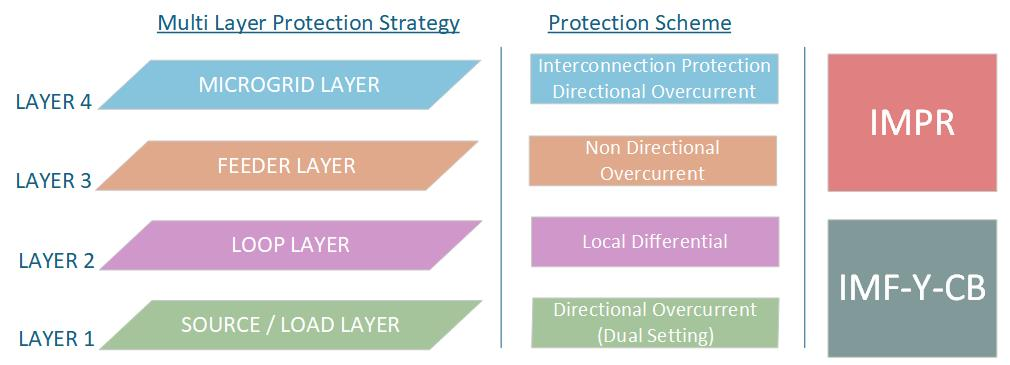
\includegraphics[width=0.95\columnwidth]{images/chapter_4/Microgrid4.jpg}
	\caption{Four-layer protection strategy , Scheme and Devices.}
	\label{fig_MG}
\end{figure}



\begin{figure}[!ht]
	\centering
    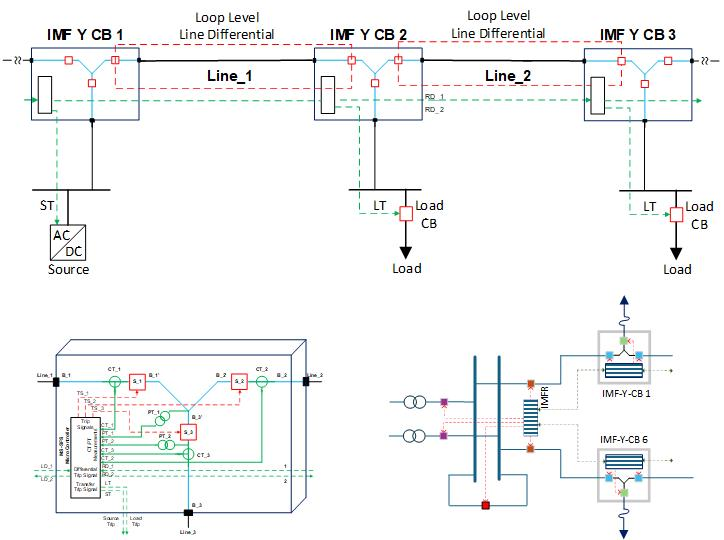
\includegraphics[width=0.95\columnwidth]{images/chapter_4/Microgrid2.jpg}
	\caption{Microgrid Protection.}
	\label{fig_MG}
\end{figure}


The load-way level shown in Fig. 5 is the basic protec-
tion element which is integrated with various DGs and loads.

The circuit in Fig. 5 includes three breakers and one DG/load, 
which can be integrated into a loop as a unit. The protection 
zones at the load-way level include Area a among break-
ers and Area b of DG/load. The loop-way level is shown in 
Fig. 6 with two types of protection: (a) short line protection 
between DGs and loads, (b) loop-way protection which can 
act as the back-up protection for both the short line protection 
and the load-way protection.
The feeder protection shown in Fig. 7 is to protect the buses 
with a similar arrangement to that of a transmission bus. The 
differential protection utilized in transmission systems can be 
directly applied in Fig. 7. The microgrid-level protection con-
siders whether or not a fault has occurred inside the microgrid, 
as discussed in the following section.


\begin{figure}[!ht]
	\centering
    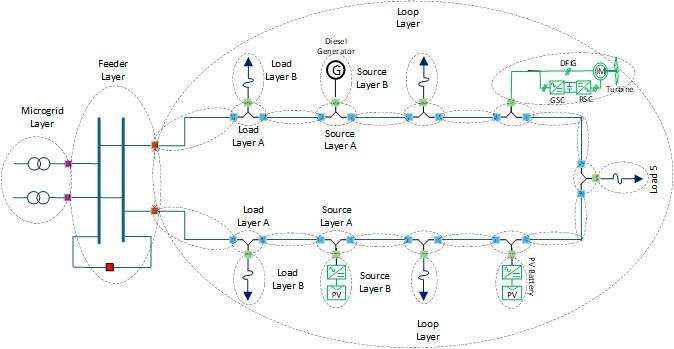
\includegraphics[width=0.95\columnwidth]{images/chapter_4/Microgrid3.jpg}
	\caption{Microgrid Protection.}
	\label{fig_MG}
\end{figure}


 




\begin{figure}[!ht]
	\centering
    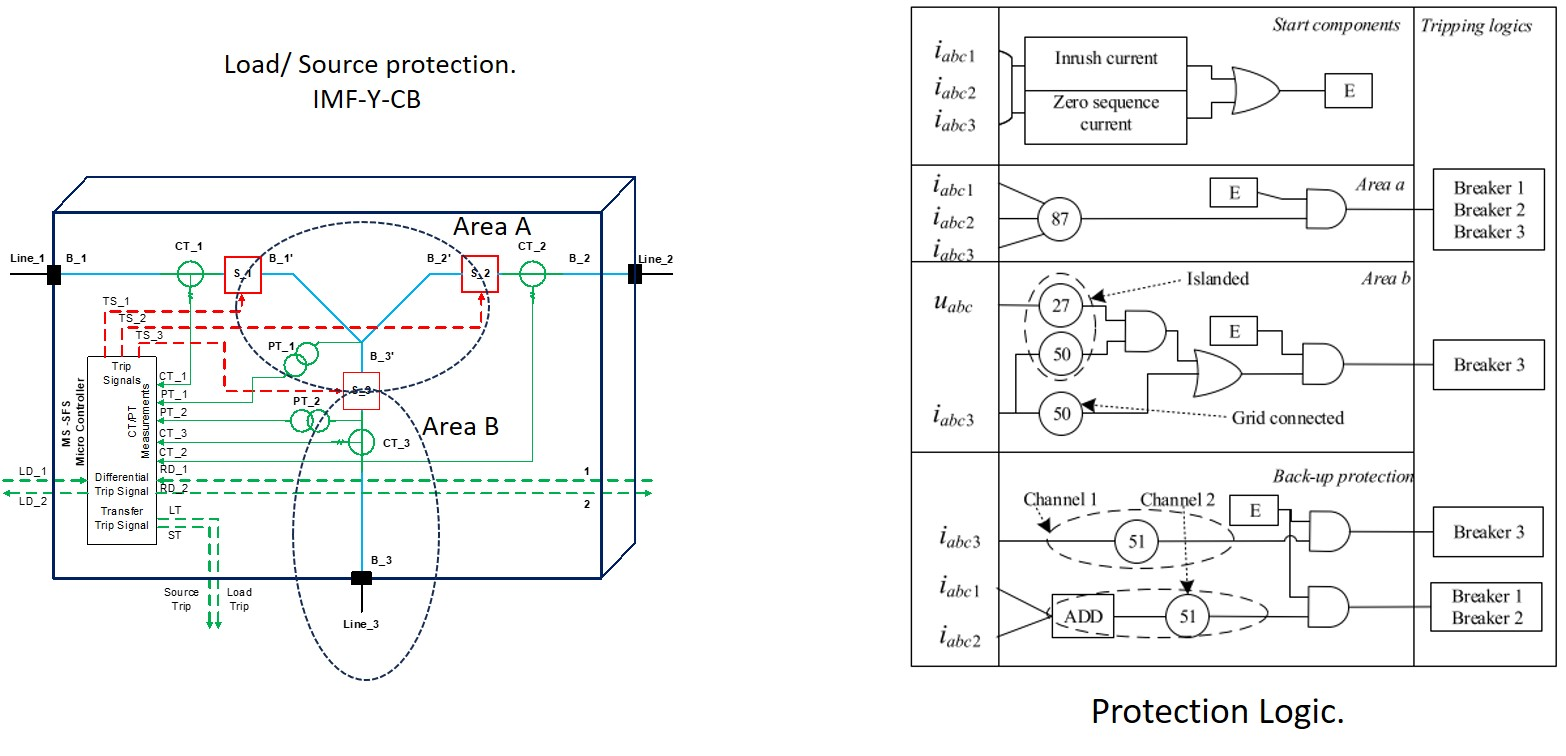
\includegraphics[width=0.95\columnwidth]{images/chapter_4/Microgrid5.jpg}
	\caption{Four-layer protection strategy , Scheme and Devices.}
	\label{fig_MG}
\end{figure}

\subsubsection{Load-Way Protection Logics}

The protection configuration of load-way module, shown in 
Fig. 8, contains three current transformers (CTs), one voltage 
transformer (VT), and three breakers. The currents iabc1 −iabc3 
in CTs and voltage uabc in VT are utilized to detect the fault in 
Areas a and b. The load-way protection logics are shown in
Fig. 9. The start components in Fig. 9 include inrush and zero
sequence currents formulated as

\begin{equation}
   \left| I_{abc} \right|_{t0+\Delta t} - \left| I_{abc} \right|_{t0} > I_{\text{set\_inrush}}
\end{equation}
\begin{equation}
   i_a + i_b + i_c > i_{\text{set\_zeroseq}}
\end{equation}

where Iabc is the root-mean-square (RMS) of iabc1, iabc2, and 
iabc3. Also, ia, ib, and ic are the instantaneous currents in 
phases a, b, and c for iabc1, iabc2, and iabc3.
Once the stated conditions for start components are satis-
fied, the protection devices in Areas a and b are enabled. The 
differential relay 87 is utilized to detect the fault in Area a,

\begin{equation}
    I_{abc1} + I_{abc2} + I_{abc3} > I_{set\_d}
    \label{eq:placeholder_label}
\end{equation}

In Area b, the island and grid-connected modes are handled 
in two ways. In the island mode, inverter-based DGs cannot 
supply enough short-circuit current (usually limited to no more 
than 1.2 times of the rated current). The under-voltage relay 
27 and instantaneous over-current relay 50 are employed to 
determine whether DG/loads lines have any faults as stated by,

\begin{equation}
    U_{abc1} < U_{set_i}
\end{equation}

\begin{equation}
    I_{abc3} > I_{set_i}
\end{equation}

In the grid-connected mode, the instantaneous over-current 
relay 50 is employed with different settings to identify the 
fault,

\begin{equation}
    I_{abc3} > I_{set_g}
\end{equation}

The instantaneous over-current settings for relay 50 in 
grid-connected and island modes are different. In the grid-
connected mode, the fault current is supplied from the utility 
which is computed using the short-circuit capacity and trans-
fer impedance. In the island mode, the short-circuit current is 
mainly supplied by inverter-based DGs.
There are two back-up protection channels. Channel 1 is 
for the failure of the primary protection of Area b in Fig. 8 
and Channel 2 is for the malfunctioning of Breaker 3. Note 
that the two channels have overlapping functions for reliability

\begin{figure}[!ht]
	\centering
    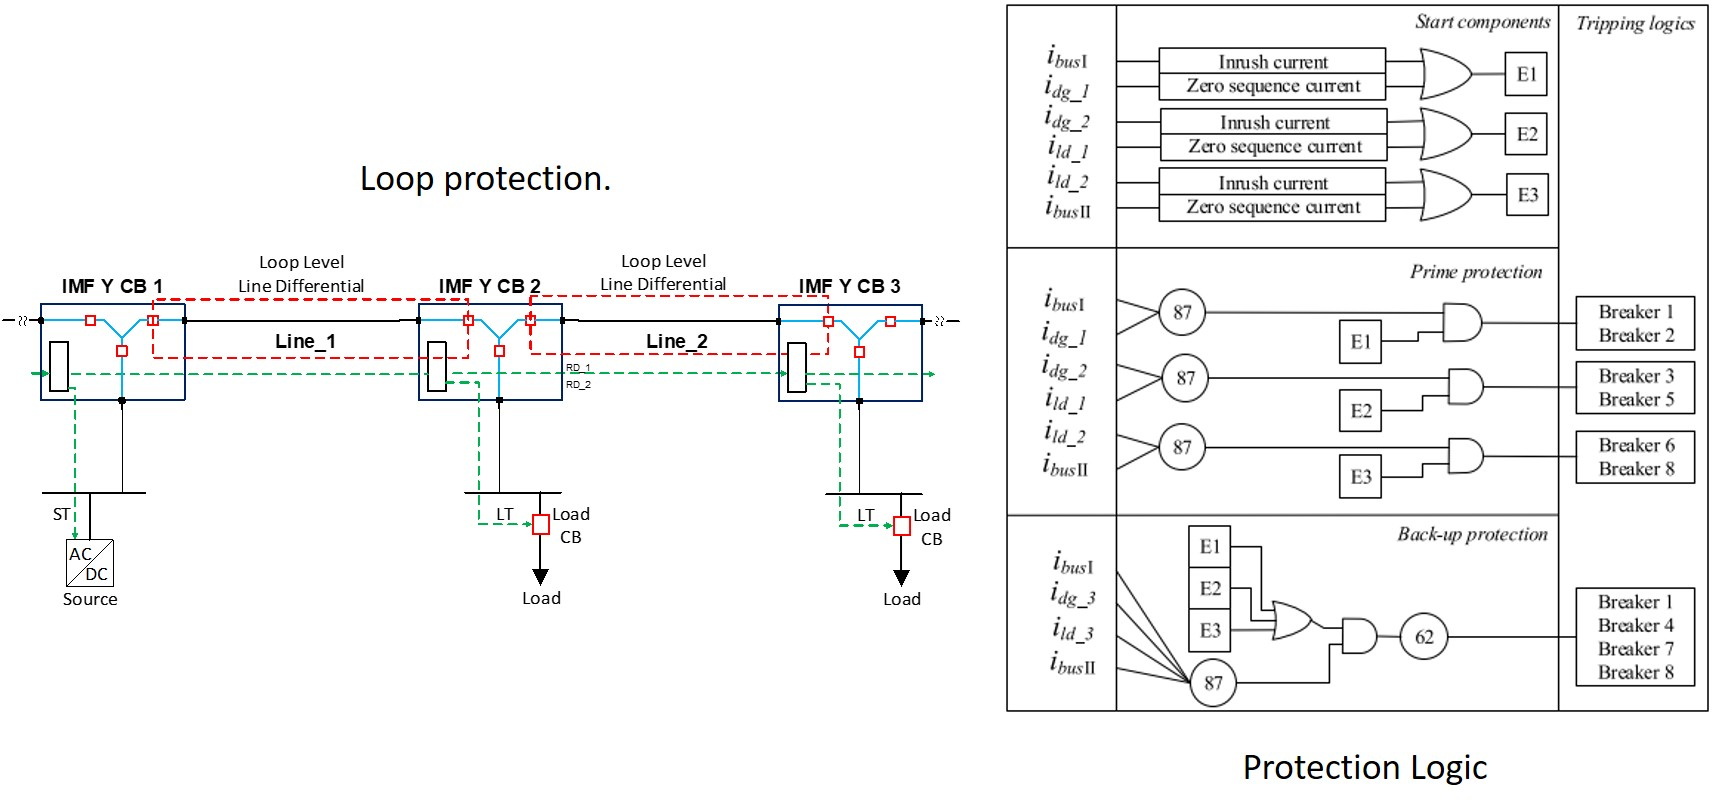
\includegraphics[width=0.95\columnwidth]{images/chapter_4/Microgrid6.jpg}
	\caption{Four-layer protection strategy , Scheme and Devices.}
	\label{fig_MG}
\end{figure}

reasons and the delay time in Channel 1 is less than that in 
Channel 2.
The over-current relay 51 is used as a back-up relay for 
failure protection in island and grid-connected modes.

\begin{equation}
    I_{abc3} > I_{set_b}
\end{equation}

The protection parameter settings in the dual strategy can 
be obtained from the dynamic simulation method, which 
can incorporate several control logics of DGs. Note that 
over-current relay settings are constrained by (8).

\begin{equation}
    I_{\text{set\_g}} > I_{\text{set\_i}} > I_{\text{set\_b}}.
    \label{eq:placeholder}
\end{equation}



\begin{figure}[!ht]
	\centering
    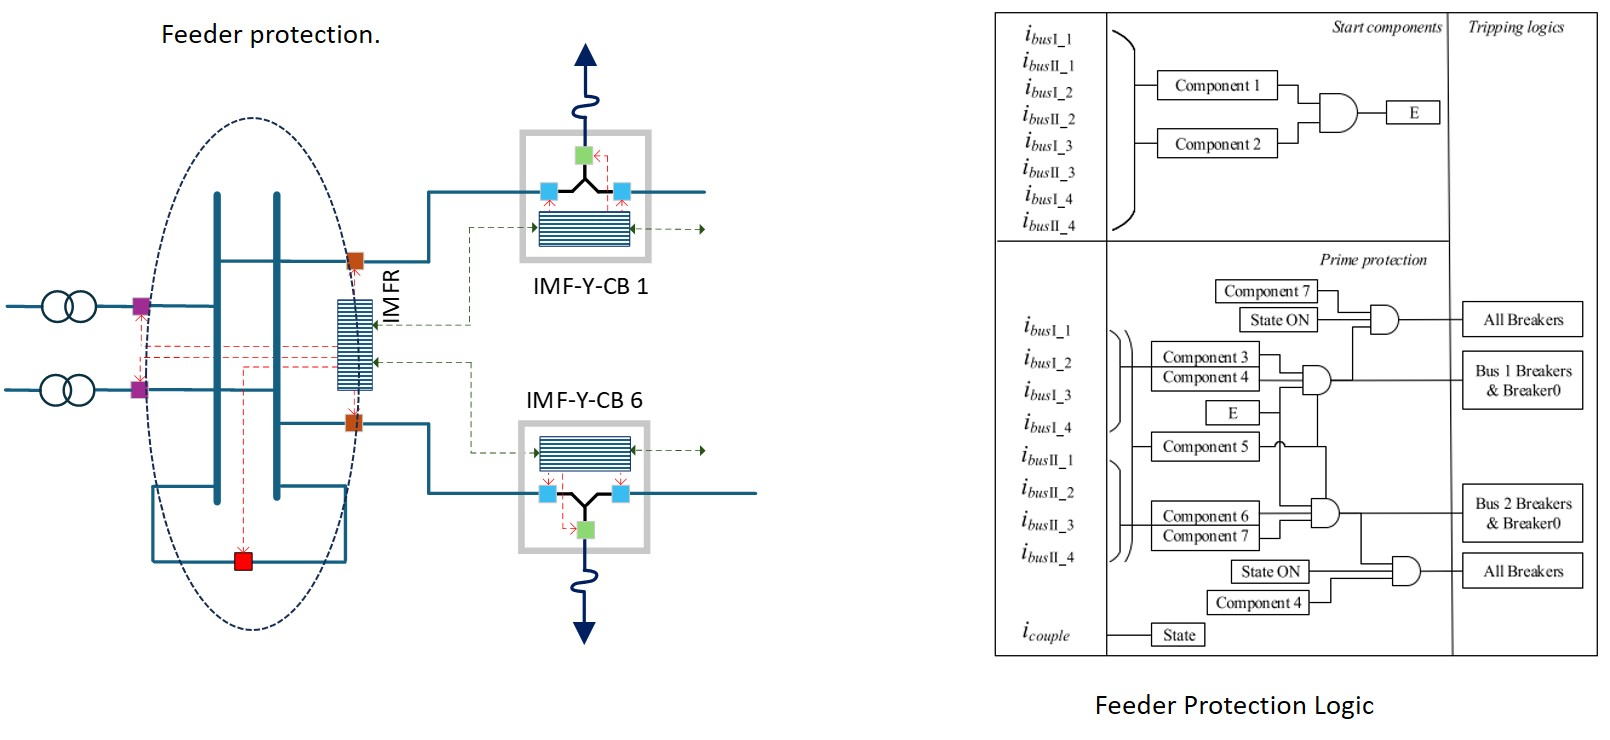
\includegraphics[width=0.95\columnwidth]{images/chapter_4/Microgrid7.jpg}
	\caption{Four-layer protection strategy , Scheme and Devices.}
	\label{fig_MG}
\end{figure}

\begin{figure}[!ht]
	\centering
    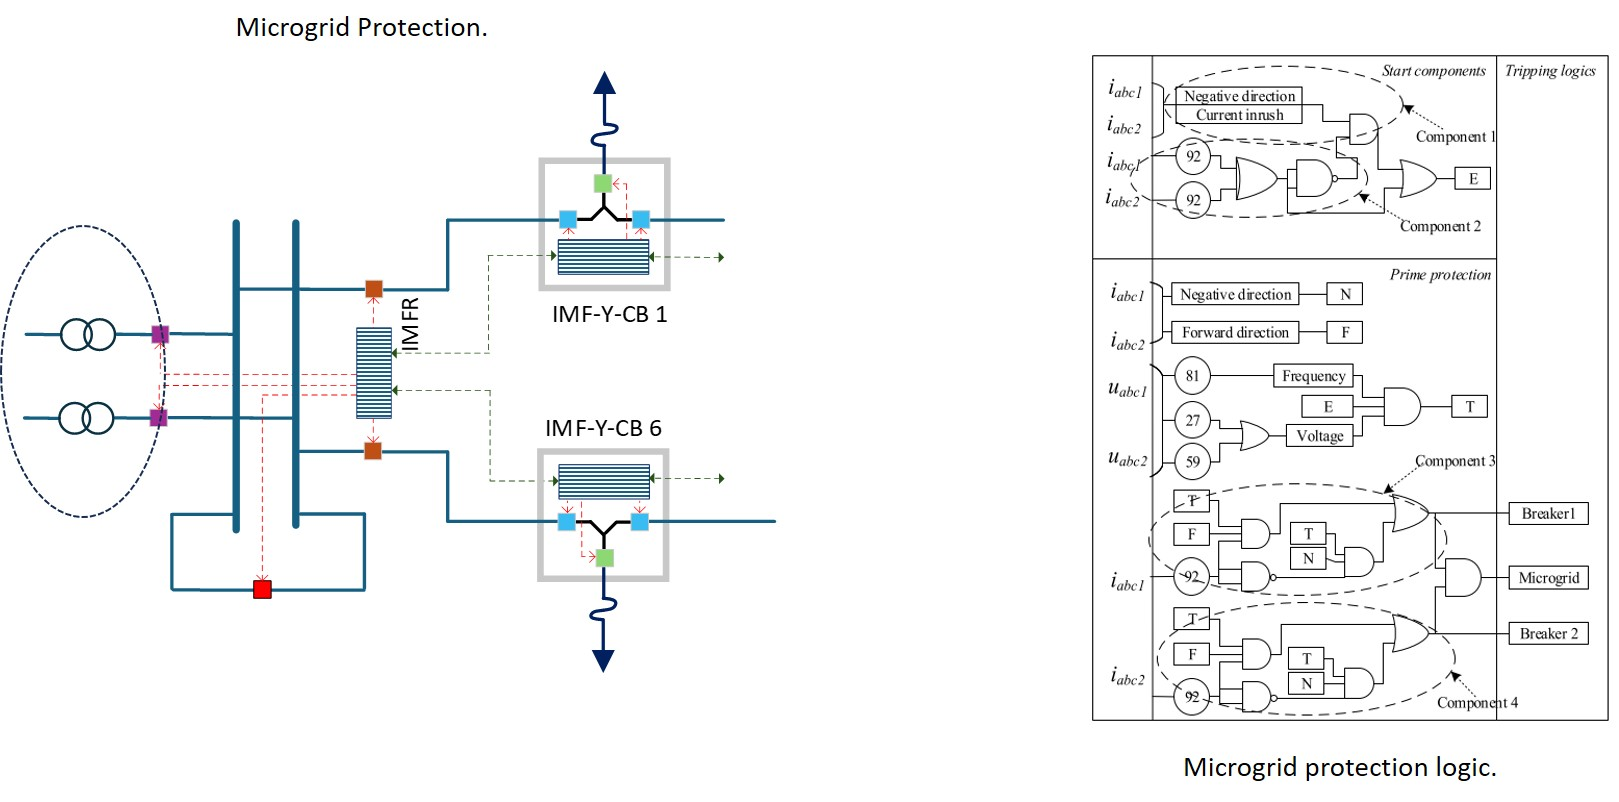
\includegraphics[width=0.95\columnwidth]{images/chapter_4/Microgrid8.jpg}
	\caption{Four-layer protection strategy , Scheme and Devices.}
	\label{fig_MG}
\end{figure}

\subsubsection{Load-Way Protection Logics}

The loop-way protection is shown in Fig. 10 in which
the differential relay 87 is utilized to protect the distribution 
cables/lines. Moreover, the plug-and-play characteristic and 
back-up protection must be involved in loop-way protections.
Suppose that a load-way unit is added in the loop shown 
in Fig. 11 where minor modifications are needed for the two-
sided differential protection. As the short-circuit current for 
the load-way unit will change especially in island mode, Iset_i 
in (8) is considered more closely. The loop-way protection
considering the plug-and-play characteristic and the backup
protection is shown in Fig. 12, which contains four differential relays and eight breakers. The protection logics for Fig. 12 are 
listed in Fig. 13.
The start components in Fig. 13 contain three enable signals 
E1, E2 and E3. Each is triggered by the inrush current or 
zero-sequence current.

% Requires: \usepackage{amsmath}
\begin{equation}
    \left| I_{abc} \right|_{t_0+\Delta t} - \left| I_{abc} \right|_{t_0} > I_{\text{set\_inrush}}
\end{equation}
\begin{equation}
    i_a + i_b + i_c > i_{\text{set\_zeroseq}}
\end{equation}

where Iabc equal to RMS of ibusI, idg_1, idg_2, ild_1, ild_2, and 
ibusII, respectively. ia, ib, and ic are phase a, b, and c of 
ibusI, idg_1, idg_2, ild_1, ild_2, and ibusII.
The primary protection contains three differential relays 87, 
and the faults which occur on lines I-III in Fig. 12 are protected 
by these relays as shown in (11)-(13). The breakers 1 and 2,
breakers 3 and 5, breakers 6 and 8 are triggered by the logics 
in primary protection

\begin{equation}
    I_{\text{busI}} + I_{\text{dg\_1}} > I_{\text{set\_d\_line}}
    \label{eq:1}
\end{equation}

\begin{equation}
    I_{\text{dg\_2}} + I_{\text{ld\_1}} > I_{\text{set\_d\_line}}
    \label{eq:2}
\end{equation}

\begin{equation}
    I_{\text{ld\_2}} + I_{\text{busII}} > I_{\text{set\_d\_line}}
    \label{eq:3}
\end{equation}

The ideal setting value of Iset-d-line is zero. However, the errors 
embedded in CTs and computer systems may actually lead to 
unbalanced differential protection systems [13]. Accordingly, 
the Iset-d-line setting depends on the CT secondary voltage rat-
ing, as well as physical wirings, relays, CT residual flux, fault 
current level, et al. In this paper, we chose (0.2 * rated current) 
as the Iset-d-line value.
The back-up protection will protect the entire line with 
differential relay 87 and time delay relay 62,




\section{Performance analysis – Case studies}.

\subsection{Results: Microgrid Example 1}.

The schematic of microgrid is illustrated in Figure which contains loop structure , a double bus arrangement, and various DGs including Diesel Generator, DFIG, PV and PV Battery. The power is supplied to various loads by the utility as well as the microgrid sources in normal grid conditions. The loop-based arrangement offers major reliability and resilience advantages. In abnormal grid conditions, the microgrid is islanded and supplied by local DGs. In a typical microgrid the short-circuit current in the grid-connected mode is dramatically different from that in the island mode because the inverter-based DGs cannot supply sufficient short-circuit currents. 

\begin{figure}[!ht]
	\centering
    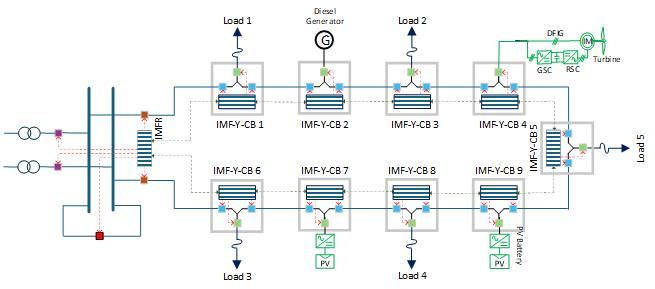
\includegraphics[width=0.95\columnwidth]{images/chapter_4/Microgrid1.jpg}
	\caption{Microgrid Protection.}
	\label{fig_MG}
\end{figure}


\subsubsection{Microgrid Protection Design}
An adaptive protection system which includes a four-level configuration is introduced, and several possible relay configurations and coordination solutions are presented in [14] for the Illinois Institute of Technology (Illinois Tech) micro-grid. Dual setting directional overcurrent relays which can handle both grid-connected and island modes are studied in [15].The scheme decomposes the protection of microgrid into four levels including load-way, loop-way, feeder, and microgrid. The protection in the load-way is achieved by a dual-strategy protection, i.e., one strategy for grid-connected and one for island modes, while the protection in the other three levels is achieved by a single-strategy protection, i.e., one strategy for both grid-connected and island modes. Each level considers DG characteristics and uti-
lizes conventional protection schemes along with protection devices. The microgrid characteristics representing plug-and-play and low-voltage-ride-through (LVRT) are taken into consideration. Also, the coordination among the four levels is discussed in this paper. The loop-based microgrid at 
Illinois Tech is considered as a testbed to study the proposed 
protection strategy. 

\begin{figure}[!ht]
	\centering
    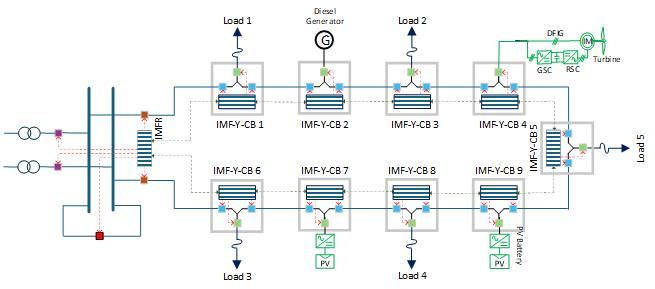
\includegraphics[width=0.95\columnwidth]{images/chapter_4/Microgrid1.jpg}
	\caption{Microgrid Protection.}
	\label{fig_MG}
\end{figure}


% \subsection{Topology of Microgrid Example 1}
% \subsection{Operational Modes}
% \subsection{Results}
% \section{Performance tesing}

\begin{figure}[!ht]
	\centering
    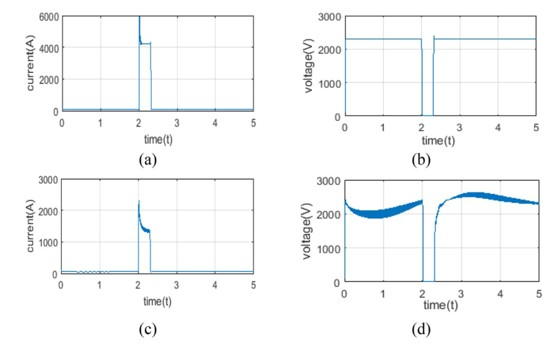
\includegraphics[width=0.95\columnwidth]{images/chapter_4/Microgrid9.jpg}
	\caption{Microgrid Protection.}
	\label{fig_MG}
\end{figure}

\begin{figure}[!ht]
	\centering
    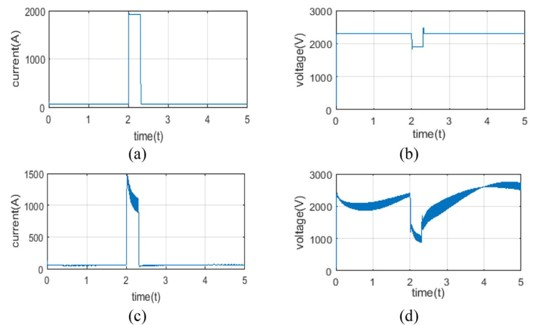
\includegraphics[width=0.95\columnwidth]{images/chapter_4/Microgrid10.jpg}
	\caption{Microgrid Protection.}
	\label{fig_MG}
\end{figure}

\begin{figure}[!ht]
	\centering
    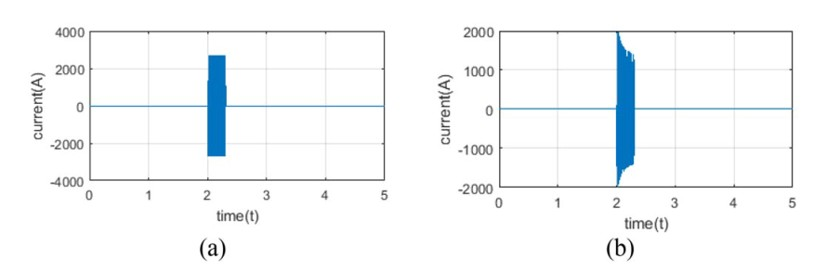
\includegraphics[width=0.95\columnwidth]{images/chapter_4/Microgrid11.jpg}
	\caption{Microgrid Protection.}
	\label{fig_MG}
\end{figure}

\begin{figure}[!ht]
	\centering
    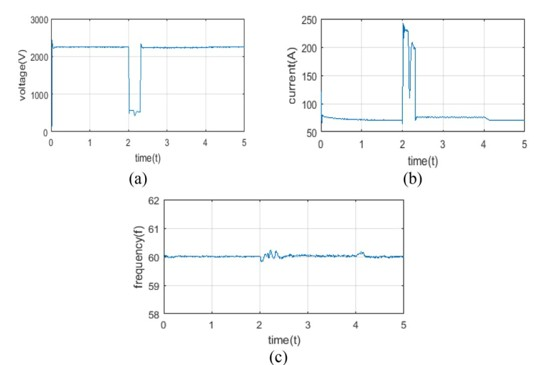
\includegraphics[width=0.95\columnwidth]{images/chapter_4/Microgrid12.jpg}
	\caption{Microgrid Protection.}
	\label{fig_MG}
\end{figure}

\begin{figure}[!ht]
	\centering
    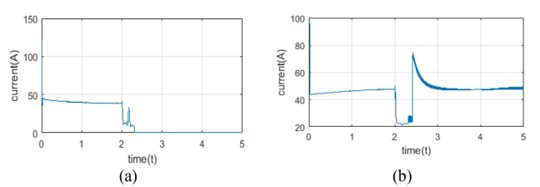
\includegraphics[width=0.95\columnwidth]{images/chapter_4/Microgrid13.jpg}
	\caption{Microgrid Protection.}
	\label{fig_MG}
\end{figure}


% \section{Results: Microgrid Example 2}.


% \subsection{Topology of Microgrid Example 2}
% \subsection{Operational Modes}
% \subsection{Results}
% \section{Performance tesing}

% \section{Results: Microgrid Example 3}.


% \subsection{Topology of Microgrid Example 3}
% \subsection{Operational Modes}
% \subsection{Results}
% \section{Performance tesing}










\begin{figure}[!ht]
	\centering
    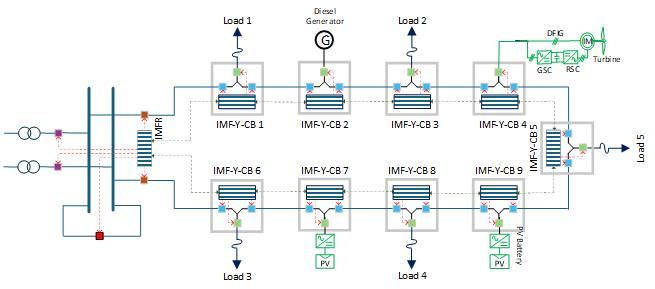
\includegraphics[width=0.95\columnwidth]{images/chapter_4/Microgrid1.jpg}
	\caption{Microgrid Protection.}
	\label{fig_MG}
\end{figure}

\begin{figure}[!ht]
	\centering
    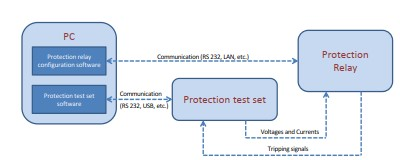
\includegraphics[width=0.95\columnwidth]{images/chapter_4/Ch5Fig1.jpg}
	\caption{Microgrid Protection.}
	\label{fig_MG}
\end{figure}

\begin{figure}[!ht]
	\centering
    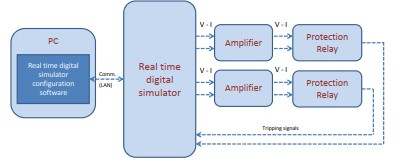
\includegraphics[width=0.95\columnwidth]{images/chapter_4/Ch5Fig2.jpg}
	\caption{Microgrid Protection.}
	\label{fig_MG}
\end{figure}


\begin{figure}[!ht]
	\centering
    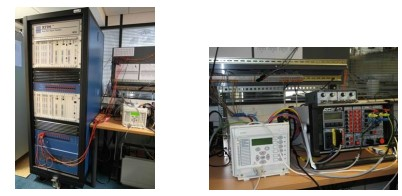
\includegraphics[width=0.95\columnwidth]{images/chapter_4/Ch5Fig3.jpg}
	\caption{Microgrid Protection.}
	\label{fig_MG}
\end{figure}

\begin{figure}[!ht]
	\centering
    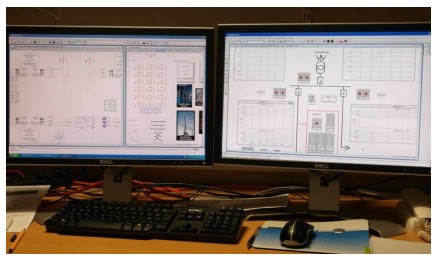
\includegraphics[width=0.95\columnwidth]{images/chapter_4/Ch5Fig4.jpg}
	\caption{Microgrid Protection.}
	\label{fig_MG}
\end{figure}

\begin{figure}[!ht]
	\centering
    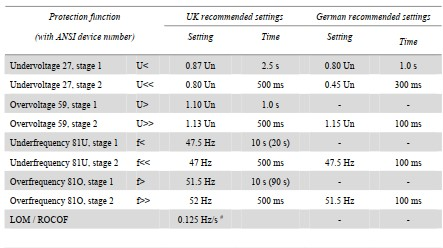
\includegraphics[width=0.95\columnwidth]{images/chapter_4/Ch5Fig5.jpg}
	\caption{Microgrid Protection.}
	\label{fig_MG}
\end{figure}

\begin{figure}[!ht]
	\centering
    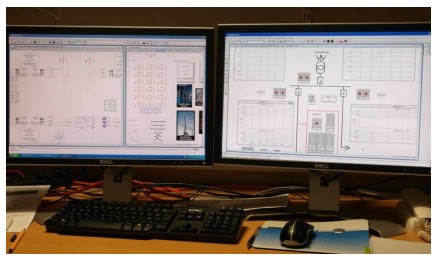
\includegraphics[width=0.95\columnwidth]{images/chapter_4/Ch5Fig4.jpg}
	\caption{Microgrid Protection.}
	\label{fig_MG}
\end{figure}


\section{Performance Testing and Results}
Three representative case studies validate the scheme:

\subsection{Microgrid Example 1: Radial AC Microgrid}
\begin{itemize}
    \item PV, BESS, diesel units; 11\,kV feeder.
    \item Fault types: SLG, LL, LLG, 3$\phi$.
\end{itemize}
Observed results:
\begin{equation}
t_{trip,51V} = 0.08\,\text{s}, \quad I_f = 1.6\,\text{pu (islanded)}
\label{eq:ex1}
\end{equation}
The differential relay operated within 70\,ms without false trips in external faults.

\subsection{Microgrid Example 2: Ring Microgrid}
GOOSE–based blocking successfully prevented sympathetic trips.  
Reduction in total trip time $\Delta t = 45$\,ms compared with conventional directional coordination.

\subsection{Microgrid Example 3: Hybrid AC–DC Microgrid}
Mode transition and resynchronisation tested under phase error $\Delta\phi < 10^\circ$, ROCOF $<0.5$\,Hz/s.
Trip coordination maintained for both AC and DC zones.

\section{Summary}
Microgrid protection must handle low, variable, and bidirectional fault currents, ensuring dependability in all modes.
The proposed four–level architecture integrates:
\begin{itemize}
    \item Voltage–assisted local relays (Level\,0)
    \item Communication–based differential/interlocking (Level\,1)
    \item Adaptive coordination via supervisory control (Level\,2)
    \item Data–driven analytics for weak–fault detection (Level\,3)
\end{itemize}
Simulation and hardware–in–loop results confirm improved speed, selectivity, and stability, enabling safe and reliable operation of inverter–dominated microgrids.






 


